\documentclass[letterpaper, margin=1in]{article}

\usepackage[english]{babel}
\usepackage[utf8]{inputenc}
\usepackage{amsmath}
\usepackage{graphicx}
\usepackage[colorinlistoftodos]{todonotes}
\usepackage{geometry}
\def\MLine#1{\par\hspace*{-\leftmargin}\parbox{\textwidth}{\[#1\]}}

\title{Crime and Punishment | final project for CAPP 30255}

\author{Carlos Grandet and Hector Salvador}

\date{\today}

\begin{document}
\maketitle

\begin{abstract}
We made a first version of a question-answering program that retrieves a set of potential answers to questions like: What is the penalty for committing murder?. We use the 300 current Mexican federal laws, specifically attempting to retrieve criminal and administrative sentences (e.g. jail years, fines, political disablement). We implement this machine in Python, using the framework described by Jurafsky and Martin \cite{jurafsky}. We show our results, challenges, and potential next steps to improve our machine.

\textbf{Keywords:} question-answering machine, natural language processing, Mexican federal laws, text analysis.
\end{abstract}

\section{Introduction}
\label{sec:introduction}

We thought a question answering machine was a good idea for a final project because:
\begin{itemize}
\item This could empower people to look if certain sentences or penalties are real. In a corrupt country like Mexico, sometimes people don't know if the punishment they're receiving is even legally sound. A lot of people would not dare to contradict a judge or a lawyer, just because they don't have any education to understand laws. 
\item It's hard to read lots of laws at once. Hector worked in the past with regulations in energy and had to quickly understand 14 new laws when they came out. This took him a very long time to read, especially since laws sometimes use a particular language and understanding them correctly takes a lot of time.
\item Since we're Mexican, we wanted to do a text analysis project in Spanish. We were very happy to  be able to apply many of the concepts we learned in class: dynamic programming, word2vec, n-gram models with Hidden Markov Models, and information retrieval (IR).
\end{itemize}


\section{Framework}
\label{sec:theory}

\subsection{Overview}

We followed the three stages of an IR-based factoid question answering machine (figure 	\ref{fig:pipeline}). We scraped 300 Mexican federal laws from the Mexican congress website\footnote{http://www.diputados.gob.mx/LeyesBiblio/index.htm}. We then used these documents to create passages (a smaller unit of documents) that would be retrieved by an IR algorithm. Finally, we prioritize these passages, using a combination of BM25 and the probability of the passage containing an answer. Because of time constraints (we had less than 1/3 of a 10-week quarter to work on this project), we could not do any work on the answer processing part of the pipeline.

\begin{figure}
\centering
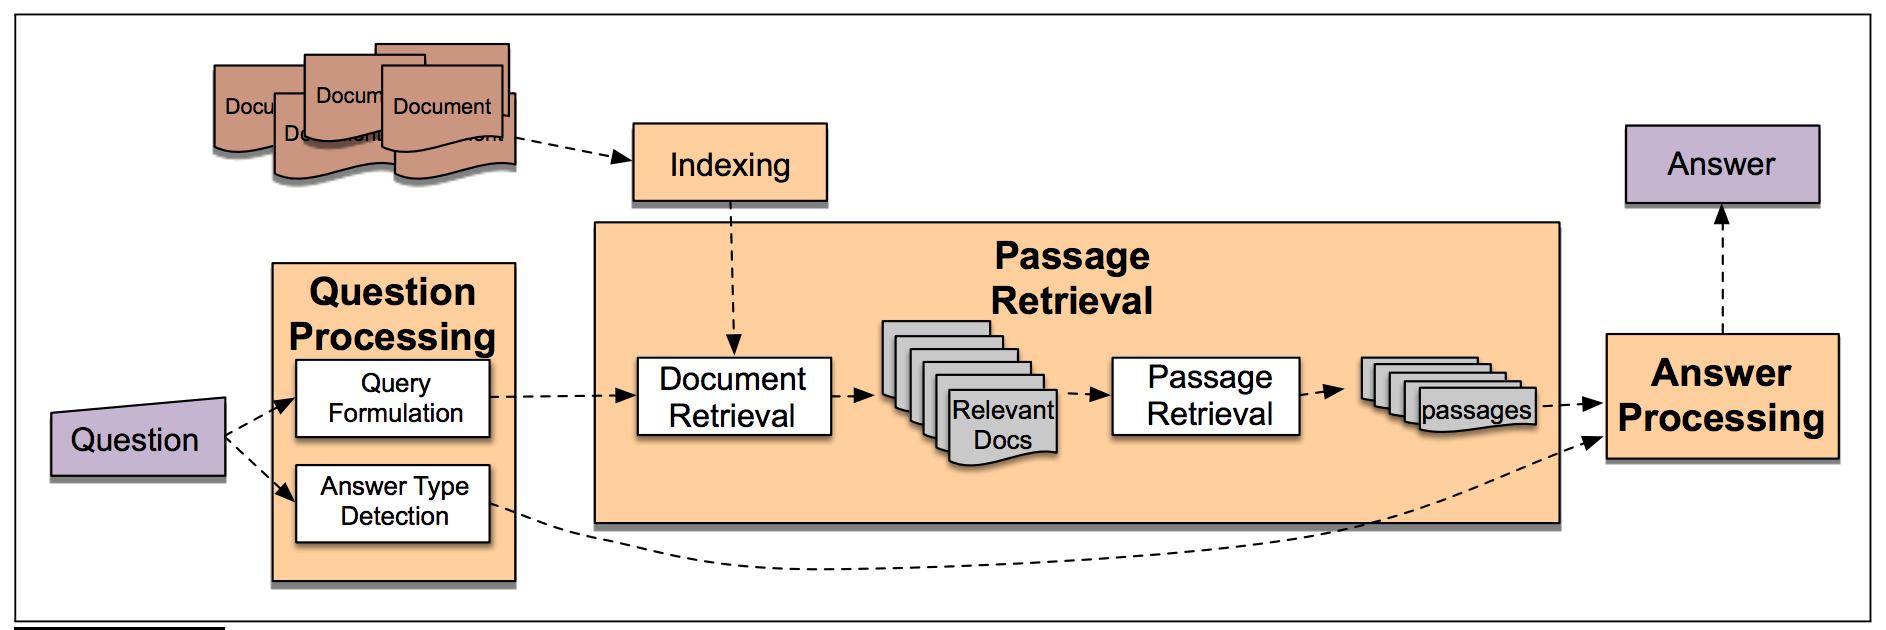
\includegraphics[width=1\textwidth]{pipeline.png}
\caption{\label{fig:pipeline}IR-based factoid question answering has three stages: question processing, passage retrieval, and answer processing. This is Figure 28.2 from \cite{jurafsky}, Chapter 28.1.1.}
\end{figure}

\subsection{Previous work}

We got inspiration from previous work on how create an answering machine

\begin{itemize}

\item Dominguez-Sal, David (2005) A Machine Learning Approach for Factoid Question Answering. This paper presents a factoid Question Answering system that is fully based on machine learning. The system achieves similar results to a state-of-the art QA system with answer extraction rules developed by a human expert. The paper uses a typical architecture consisting of three components linked sequentially: Question Processing (QP), which identifies the type of the put question, followed by Passage Retrieval (PR), which extracts a small number of relevant passages from the underlying speech transcriptions, and finally Answer Extraction (AE), which extracts and ranks exact answers from the previously retrieved passages. It has a similar pipeline than Jurafsky and Martin (2016) which was reassuring, although, it mainly relies on Maximum Entropy multiclass classifier to do the question and answering processing.

\item  Strohn, Eylon. (2015) Question Answering Using Deep Learning. The paper proposes the application of several deep learning models to the question answering tasks. It particularly focuses on recurrent neural networks-based baselines. The idea is to propose a different idea than the conventional linguistically-based NLP techniques, such as parsing, part-of-speech tagging and coreference resolution.

\item  Florent Jousse, Isabelle Tellier, Marc Tommasi and Patrick Marty (2014) Learning to Extract Answers in Question Answering: Experimental Studies. The main objective of this study it to adapt machine learning techniques defined for Information Extraction tasks to the slightly different task of answer extraction in QA systems. The specificities of QA systems are identified and exploited in this adaptation. Three algorithms, assuming an increasing abstraction of natural language texts, are tested and compared.

\item 

\end{itemize}


\subsection{Document creation}
Scraping was done using \texttt{scrape.py}. Laws were available both in \texttt{pdf} and \texttt{doc} files. Two methods were tested to convert the files to \texttt{txt} files that could be processed in Python. 

First we tried converting \texttt{pdf} files to \texttt{txt} using out-of-the-box packages (e.g. using \texttt{pdftotext} utility in the command line). Unfortunately, Mexican laws have a ton of useless text as headers and footnotes \ref{fig:header}, which are repeated over all documents. This introduced a lot of noise in our models, so we tried next using \texttt{doc} files.

We attempted unsuccessfully to just open \texttt{doc} files in Python. There were a lot of binary characters that made reading and text processing difficult. Maybe it was our lack of experience opening files, but we could not find a way to retrieve only the text we needed, especially since many characters have accents in Spanish. We also tried using \texttt{antiword} and \texttt{python-docx}, but we kept having installation errors, even using a virtual environment\footnote{Using a macOS Sierra 10.12.3 and python 3.5}.

After spending several hours, we opted to manually convert \texttt{doc} files to \texttt{txt} manually. These can all be found in the folder called \texttt{/leyes/*}.

\begin{figure}
\centering

\includegraphics[width=1\textwidth]{header.png}
\caption{\label{fig:header}Example of the top part of a Mexican Law saved as a doc file. Notice the headers, the titles, subtitles, and additional text that is non-informative.}
\end{figure}

\subsection{Question processing}
To conduct the question processing we followed three steps:

\begin{itemize} 

\item Phrase tagging, we created a class that tagged words in spanish called Spanish_Postagger (found in \texttt{spanish_tagger.py}) and we use the Stanford lexical and grammatical rules to train this class into being able to classify correctly each word according to it being a pronoun, noun, verb. The idea of doing this was to tag each word of the question that was being asked in order to recognize which are the relevant queries of the question. 

Additionally, in order to control for common words, we used a dictionary of stop words  that can be found in \texttt{stopwords.json}

\item Finding common words, the next part of the project was finding similar
concepts or synonyms for the words that were part of the question. Sometimes
there can be an issue when you are not asking the appropiate term for a legal
procedure and the work could not be found in the laws. That's why we devised
two mechanisms through which the query could find new, similar concepts. 

The first of this mechanisms was using a Word2Vec model, the Word2Vec model
was trained using a library called gensim which allows to load Word2Vec models and ask for simmilarity and perform linear algebra to find concepts.
We created a class called W2V (found in \texttt{Word2VecModel.py}) and load it with a vector model found in http://crscardellino.me/SBWCE/

The corpus used the following data

\begin{itemize} 
\item Spanish portion of SenSem.
\item Spanish portion of the Ancora Corpus.
\item Tibidabo Treebank and IULA Spanish LSP Treebank.
\item The Spanish portion of the following OPUS Project Corpora:
\item The books aligned by Andras Farkas.
\item The JRC-Acquis collection of legislative text of the European Union.
\item The News Commentary corpus.
\item The United Nations documents compiled by Alexandre Rafalovitch and Robert Dale.
\item The Spanish portion of the Europarl (European Parliament), compiled by Philipp Koehn.
\item Dumps from the Spanish Wikipedia, Wikisource and Wikibooks on date 2015-09-01, parsed with the Wikipedia Extractor.
\end{itemize} 

The second mechanism was to use an API from https://store.apicultur.com/, 
that allowed us to query for synonyms. We created a class called Synonyms in the \texttt{synonyms.py} code that fetched synonyms. 

\item The third part was a question processing class that took a question transformed it into a query and assigned a question type. To assign the question type we used a dictionary of words
called \texttt{question_type.json} that showed as keys the possible types of questions 
and as values the possible words that could related to this type of key. In this case there
were only two types of questions: time in jail or monetary penalty and we simply used all words we could find related to these concepts with both the Word2Vec model and the synonyms API. We used a probability model to determine which was the most likely question type. We called the class Question and it is in the \texttt{question_processing.py} file.


In the end we used all of this classes to create one super class called Query in the \texttt{query.py} file that allowed you to initiate a query script in which you loaded all of the relevant classes: word2vec, stanford postagger and synonyms API, asked questions and got answers. 

\end{itemize} 

\subsection{Document retrieval}
The document retrieval part had two steps: first create indices and store them on disk, then do the actual querying. For the first step, we built an inverted index where keys were words and values were names of laws containing an occurrence of such word. We also made such an index for every law, where we could find the article number containing a specific word.  These indices can be built using the python file called \texttt{index.py}. 

For the querying step, we also took two steps: first look for documents where it was possible to find an answer, then scoring retrieved passages to determine which ones seemed to have an answer. The first search just employed inverted indices, identifying documents where at least one of the terms of our search appeared. Finally, to score our passages we employed a mix of the BM25 algorithm and a 3-gram model with Naive Bayes; this 3-gram model attempted to predict which passages were the most likely to be actually passages containing penalties or sanctions.

It is important to note that words were stemmed for this exercise using the Spanish stemmer from the  \texttt{nltk} library. We also avoided stop words, which were manually filtered after getting the most frequently occurring words in the corpus. To separate laws into their corresponding articles, we used regular expressions. Encoding text files previously was really useful, as diacritics in Spanish were very easy to match using UTF-8 encoding and regex. 

For the scoring we tried different methods, including:

\begin{itemize}
\item Jaro-Winkler distance of the original query with the passage.
\item Count of terms in the query appearing in the passage.
\item TF-IDF
\end{itemize}

Unfortunately, none of them seemed to provide useful results by itself. But when we added the extra filter with the n-gram model, results started to make more sense. This 3-gram model was trained using a manually constructed database of articles that contained information on penalties, sanctions, and fines from a variety of laws. We also used a database containing counterexamples of texts that did not have any type of penalties on them. We would finally take the probabilities of being a sentence passage (label 1) or not (label 0), and get a ratio as a score. 

\section{Results}
We did not have metrics for this exercise, as we didn't have a labeled dataset to test questions. We manually checked for the coherence of top results, using three main questions:
\begin{itemize}
\item Cual es el castigo por homicidio? (\textit{What is the punishment for murder?})
\item Cual es el castigo por el robo de hidrocarburos? (\textit{What is the punishment for stealing hydrocarbons?})
\item Cual es el castigo por no pagar impuestos? (\textit{What is the punishment for not paying taxes?})
\end{itemize}


We got mixed results for these questions.An example of an answer about punishment for murder is shown below, it refers to death by reckless driving. 

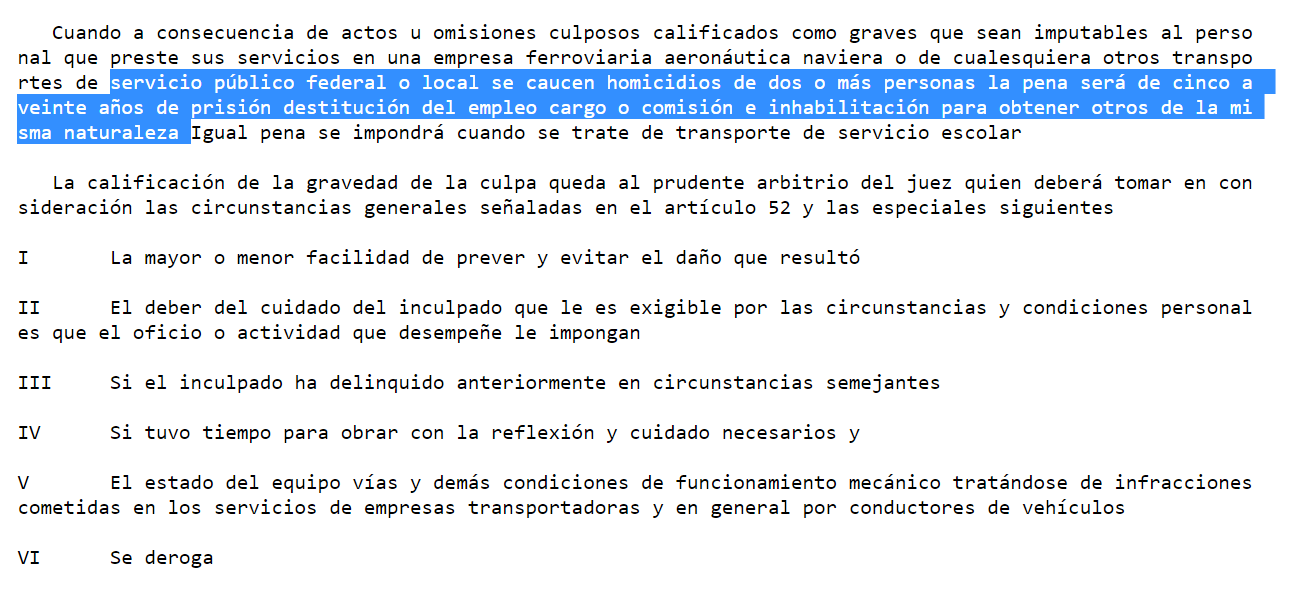
\includegraphics[width=1\textwidth]{Result.png}

\image{} 

Overall, we are still far from retrieving the exact articles that contain answers for our questions. We analyze some of the reasons we believe this is happening. \\

For the query corresponding to the first question, \textit{What is the punishment for murder?}, we obtained the following articles:
\begin{itemize}
\item In cases of wrongful misdemeanor, up to one quarter of the penalties and security measures assigned by law to basic type of criminal offenses, with exception of those for which the law specifies a specific penalty, will be imposed. Additionally, if corresponding, it will be imposed the suspension of up to three years of license to work on their corresponding profession. [...]
\item The judge will void the substitution and will order the execution of prison penalty previously imposed when the sentenced doesn't comply with the conditions ordered for such effect, except when the judge esteems convenient to warn the sentenced that if a new fault is observed or is condemned by a new criminal offense, the sanction will be made effective. [...]
\item Technical or artistic professionals and their auxiliaries will be responsible for the crimes they might commit in the exercise of their profession [...]: \\
Additional to the fixed sanction for the felonies consummated, depending on whether offenses are wrongful misdemeanor or criminal offenses, a suspension of one month up to two years will be applied or up to definitive suspension in the case of recidivism. [...]
\item Prison of three day up to two years or 30 to 90 days of fine will be imposed to: \\
I. Whomever hides, destroys, or buries a corpse or human fetus without the order of the authority who corresponds, or without the requisites stipulated by the Civil Code and Health Code or special laws. \\
II. [...]
\end{itemize}

We can identify that it is only in the last result where we have explicit penalties for crimes. Nevertheless, these do not correspond directly to murder or homicide, but rather to burying dead corpses. Although related, not the same concept. The other results talk about criminal offenses and wrongful misdemeanors, these are categorizations, and murder fall into one of these, depending on the intention of the murderer. 

For the following two questions, we got unusual results. Sometimes these would refer to laws that were quite unrelated to our point of interest, such as the hydrocarbons query which gave results from laws that were about immigration. 
 
\subsection{Further Work}
There are possibilities of improvement in all the sections of our work. The first and most important would be to create a test dataset with some example questions for which we know exactly which articles are relevant. Since neither of use are lawyers, we could only use our best judgement to determine which seemed to be sensible results. But after having a useful test set, we could do the following improvements.
\begin{description}
\item \textbf{Document processing:} improve the pipeline to convert \texttt{doc} to \texttt{txt} files.
\item \textbf{Question processing:} we need to train a w2v model with the Mexican laws to have better accuracy.
\item \textbf{Document retrieval:} test other methods for passage retrieval (e.g. proximity), and other parameters for the tested ones (e.g. use a 4-gram or higher-gram model). It could also be useful to make a more specific document retrieval, based on the whole query, and not individual words.
\item \textbf{Answer processing:} actually develop a script that takes a long passage and returns only the amount of information related to the sanction, penalty, or fine
\end{description}

\newpage
\section{How to run the code}

\subsection{Dependencies}
\begin{itemize}
\item requests, bs4, for the scraping
\item synonyms
\item gensim 
\item nltk, for stem.snowball.SpanishStemmer, tokenize.RegexpTokenizer, tag.StanfordPOSTagger
\item textblob, for easy word manipulation
\item jellyfish, for Jaro-Winkler sitance
\item sklearn, for general processing, including TF, IDF, and Multinomial Naive Bayes models
\item numpy, pandas

\end{itemize}

\subsection{Instructions}
Before running the code, make sure that the \texttt{txt} files are in folder called leyes and that the file called \texttt{docnames.csv} is in the folder called \texttt{doc}. Remember also to add the stanford postagger (\texttt{stanford-postagger-full-2016-10-31}) in the root directory and the word2vec file (\texttt{SBW-vectors-300-min5.txt}) in the \texttt{Data} folder.

\begin{enumerate}
\item Open a Python shell, preferably ipython.
\item If you want to download the \texttt{doc} files, run \\ \texttt{\$ run scrape.py} \\ \texttt{\$ go()} \\ This will download the \texttt{doc} files in the folder called \texttt{/doc}.
\item Create the indices by running \\ \texttt{\$ run index.py} \\ \texttt{\$ go()}
\item Run a query with a sentence specified in \texttt{query.py}
\end{enumerate}

Alternatively, you can use the \texttt{jupyter notebook} titled \texttt{QA{\_}machine}, available in the root directory of the repository.

\begin{thebibliography}{9}
\bibitem{jurafsky}
  Jurafsky, Dan, and James H. Martin. 
  \emph{Speech and language processing: an introduction to natural language processing, computational linguistics, and speech recognition.} 
  India: Dorling Kindersley Pvt, Ltd., 2014.
\bibitem{Jousse}
 Florent Jousse, Isabelle Tellier, Marc Tommasi and Patrick Marty (2014) Learning to Extract Answers in Question Answering: Experimental Studies
\bibitem{Sal}
 Dominguez-Sal, David (2005) A Machine Learning Approach for Factoid Question Answering.
\bibitem{Strohn}
Strohn, Eylon. (2015) Question Answering Using Deep Learning. 

\end{thebibliography}

\newpage
\appendix

\section{Repository structure}
The repository has the following folders:
\begin{itemize}
\item \texttt{Data}
\item \texttt{doc}
\item \texttt{indices}
\item \texttt{leyes}
\item \texttt{stanford-postagger-full-2016-10-31}
\end{itemize}

It also has a bunch of Python scripts and miscellaneous files:

\begin{itemize}
\item \texttt{scrape.py}
\item \texttt{index.py}
\item \texttt{ngrams.py}
\item \texttt{query.py}
\item \texttt{question{\_}processing.py}
\item \texttt{retrieval.py}
\item \texttt{spanish{\_}tagger.py}
\item \texttt{synonyms.py}
\item \texttt{Word2VecModel.py}
\end{itemize}

The data sources are the following 
\begin{itemize}
\item Stanford Postagger - https://nlp.stanford.edu/software/tagger.shtml
\item Word2Vec - http://crscardellino.me/SBWCE/
\item Laws - http://www.diputados.gob.mx/LeyesBiblio/index.htm
\end{itemize}

The time spent in project is the following
\begin{itemize}
\item Literature Review - 8 hours 
\item Scrapping Data - 6 hours 
\item Processing data - 4 hours
\item Question Processing 24 hours 
\item Text retrieval - 20 hours 
\end{itemize}

The lines of code contributed by team member
\begin{itemize}
\item Hector Salvador - scrape.py, retrieval.py, index.py, QA_machine.ipynb (500 lines of code)
\item Carlos Grandet - synonyms.py, spanish_tagger.py, query.py, question_processing.py,
Word2VecModel.py, QA_machine.ipynb (500 lines of code)
\end{itemize}

Miscellaneous:
\begin{itemize}
\item \texttt{get{\_}l.sh}: count average document length to use in BM25 algorithm.
\end{itemize}

\end{document}